\documentclass[a4paper,11pt]{jsreport}

\usepackage{comment}
\usepackage{float}
\usepackage{color}
\usepackage{multicol}
\usepackage[dvipdfmx]{graphicx}
\usepackage{wrapfig}
\usepackage{graphicx}
\usepackage{bm}
\usepackage{url}
\usepackage{underscore}
\usepackage{colortbl}
\usepackage{tabularx}
\usepackage{fancyhdr}
\usepackage{ulem}
\usepackage{cite}
\usepackage{amsmath,amssymb,amsfonts}
\usepackage{algorithmic}
\usepackage{textcomp}
\usepackage{xcolor}
\usepackage[ipaex]{pxchfon}


\begin{document}

\thispagestyle{empty}
\begin{center}

  \vspace{20mm}
  {\Large\noindent 2024年度 修士論文}\\
  \vspace{40mm}
  {\Huge\noindent\textbf{機械学習を用いた}}\\
  \medskip
  {\Huge\noindent\textbf{イジング模型の臨界現象に関する研究}}\\
  \vspace{\baselineskip}
  \vspace{40mm}

  {\Large\noindent
    2024年2月00日\\
    \vspace{\baselineskip}
    指導教員 \ 藤原高徳    \\
    \vspace{\baselineskip}
    茨城大学大学院\\
    理工学研究科 \ 量子線科学専攻 \\
    \vspace{\baselineskip}
    学籍番号 \ 22NM021S \\
    氏名 \ 須賀 勇貴\\
  }
  \vspace{40mm}

\end{center}

\thispagestyle{empty}
\clearpage

%=====================================================================================
\renewcommand{\abstractname}{要旨}

\begin{abstract}
  研究の要旨を書く.
\end{abstract}

\thispagestyle{empty}
\clearpage

%=====================================================================================

% 目次の表示
\tableofcontents

%=====================================================================================
\pagestyle{fancy}
\lhead{\rightmark}
\renewcommand{\chaptermark}[1]{\markboth{第\ \normalfont\thechapter\ 章~~#1}{}}
%=====================================================================================
\chapter{はじめに} %章
\section{研究背景}
\section{研究目的}


\chapter{イジング模型の数理}
\section{イジング模型とは}
\section{自由エネルギー}

\chapter{機械学習と深層学習}
ここでは,イジングモデルに対して機械学習,深層学習による手法を応用する上で必要となる機械学習と深層学習の基礎知識について説明する.
\section{機械学習の定義}
機械学習(machine learning)とは,人間がこなすような学習や知的作業を計算機に実行させるためのアプローチの研究,あるいはその手法そのもののことを意味する.機械学習では,知識を人間が直接アルゴリズムに具体的に書き込んだり教え込んだりせず,データという具体例の集まりから計算機に自動的に学ばせるという方法をとる.\par
機械学習の定義としてT. M. ミッチェル(Tom Michael Mitchell)の書籍\cite{Tom1997Machine}で書かれている定義が有名である.それは
\begin{quote}
  "コンピュータプログラムが,ある種のタスクTとパフォーマンス評価尺度Pにおいて,経験Eから学習するとは,タスクTにおけるその性能をPによって評価した際に,経験Eによってそれが改善されている場合である."
  \hfill T. M. ミッチェル
\end{quote}
である.ここで,タスクTとは解きたい問題のこと,パフォーマンス評価尺度Pは精度,誤差率などの評価指標のこと,経験Eはデータセットのことを指す.\par
機械学習では,何かしらのモデルを構築する必要がある.このモデルというのは,なにかしらの入力が与えられたときに出力を返すものであり,その正体は多数のパラメータを持った非線形関数$f_{\bm{\theta}}(\bm{x}), \ \bm{\theta} = \{ \theta_1, \theta_2, \theta_3, \cdots \}$である.
\begin{figure}[b]
  \begin{center}
    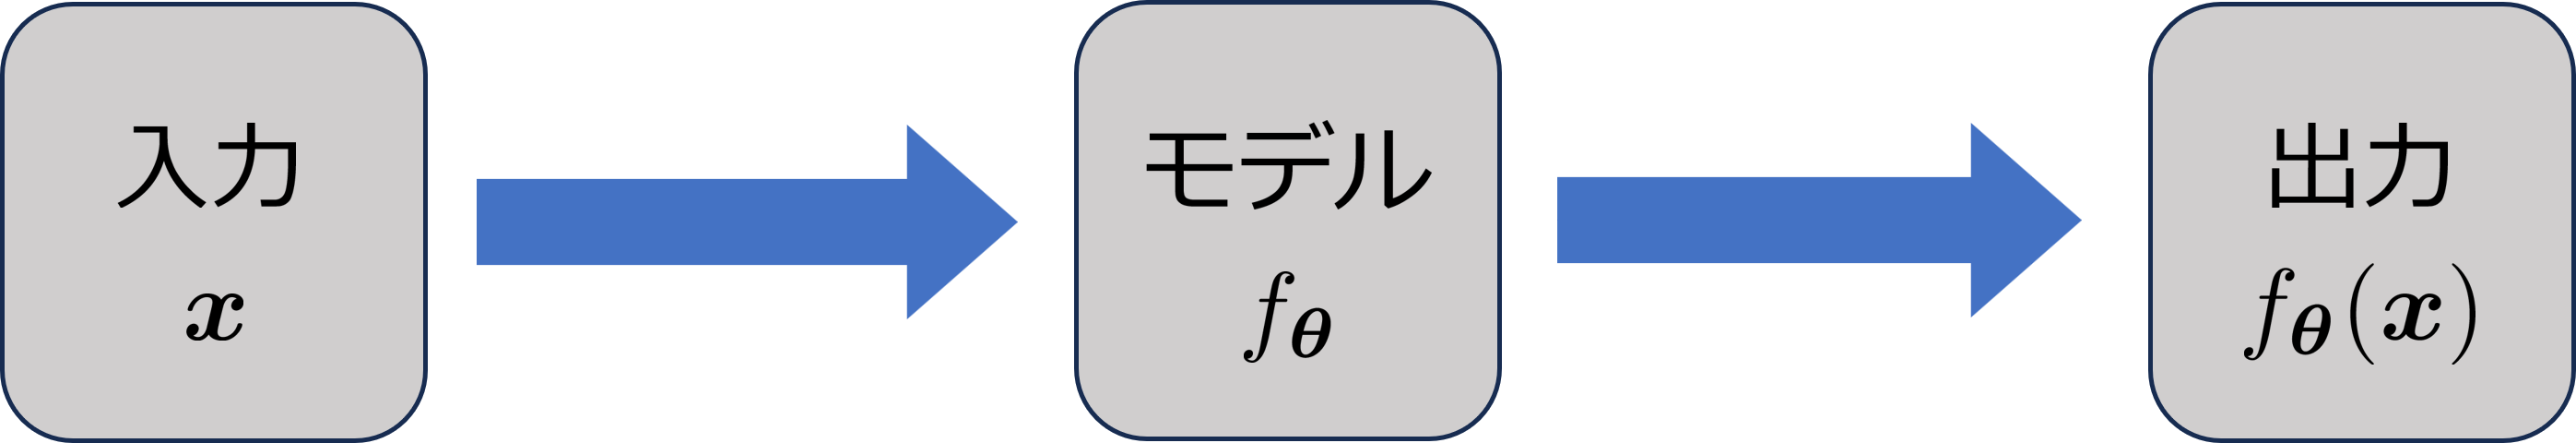
\includegraphics[height=1.5cm]{image/モデル概略図.png}
    \caption{モデルの概略図}
  \end{center}
\end{figure}
このパラメータの値は最初はランダムに初期化されており,入力を与えると出力が返ってくるが,このときの出力結果は本来出力してほしい正解の値からは外れた値が帰ってくる.そこで,出力と正解の誤差を測るような評価基準を決めておき,算出された評価結果を良くするようにモデルのパラメータを更新してあげることによってモデルを改善していく.この一連の流れを繰り返し行うことで,モデルを改善して,正解に近い出力結果を得られるモデルを作成すること機械学習とよぶ.ここで注目してほしいのは,機械学習ではモデルの改善を機械に行わせているという点である.\par
\begin{figure}[t]
  \begin{center}
    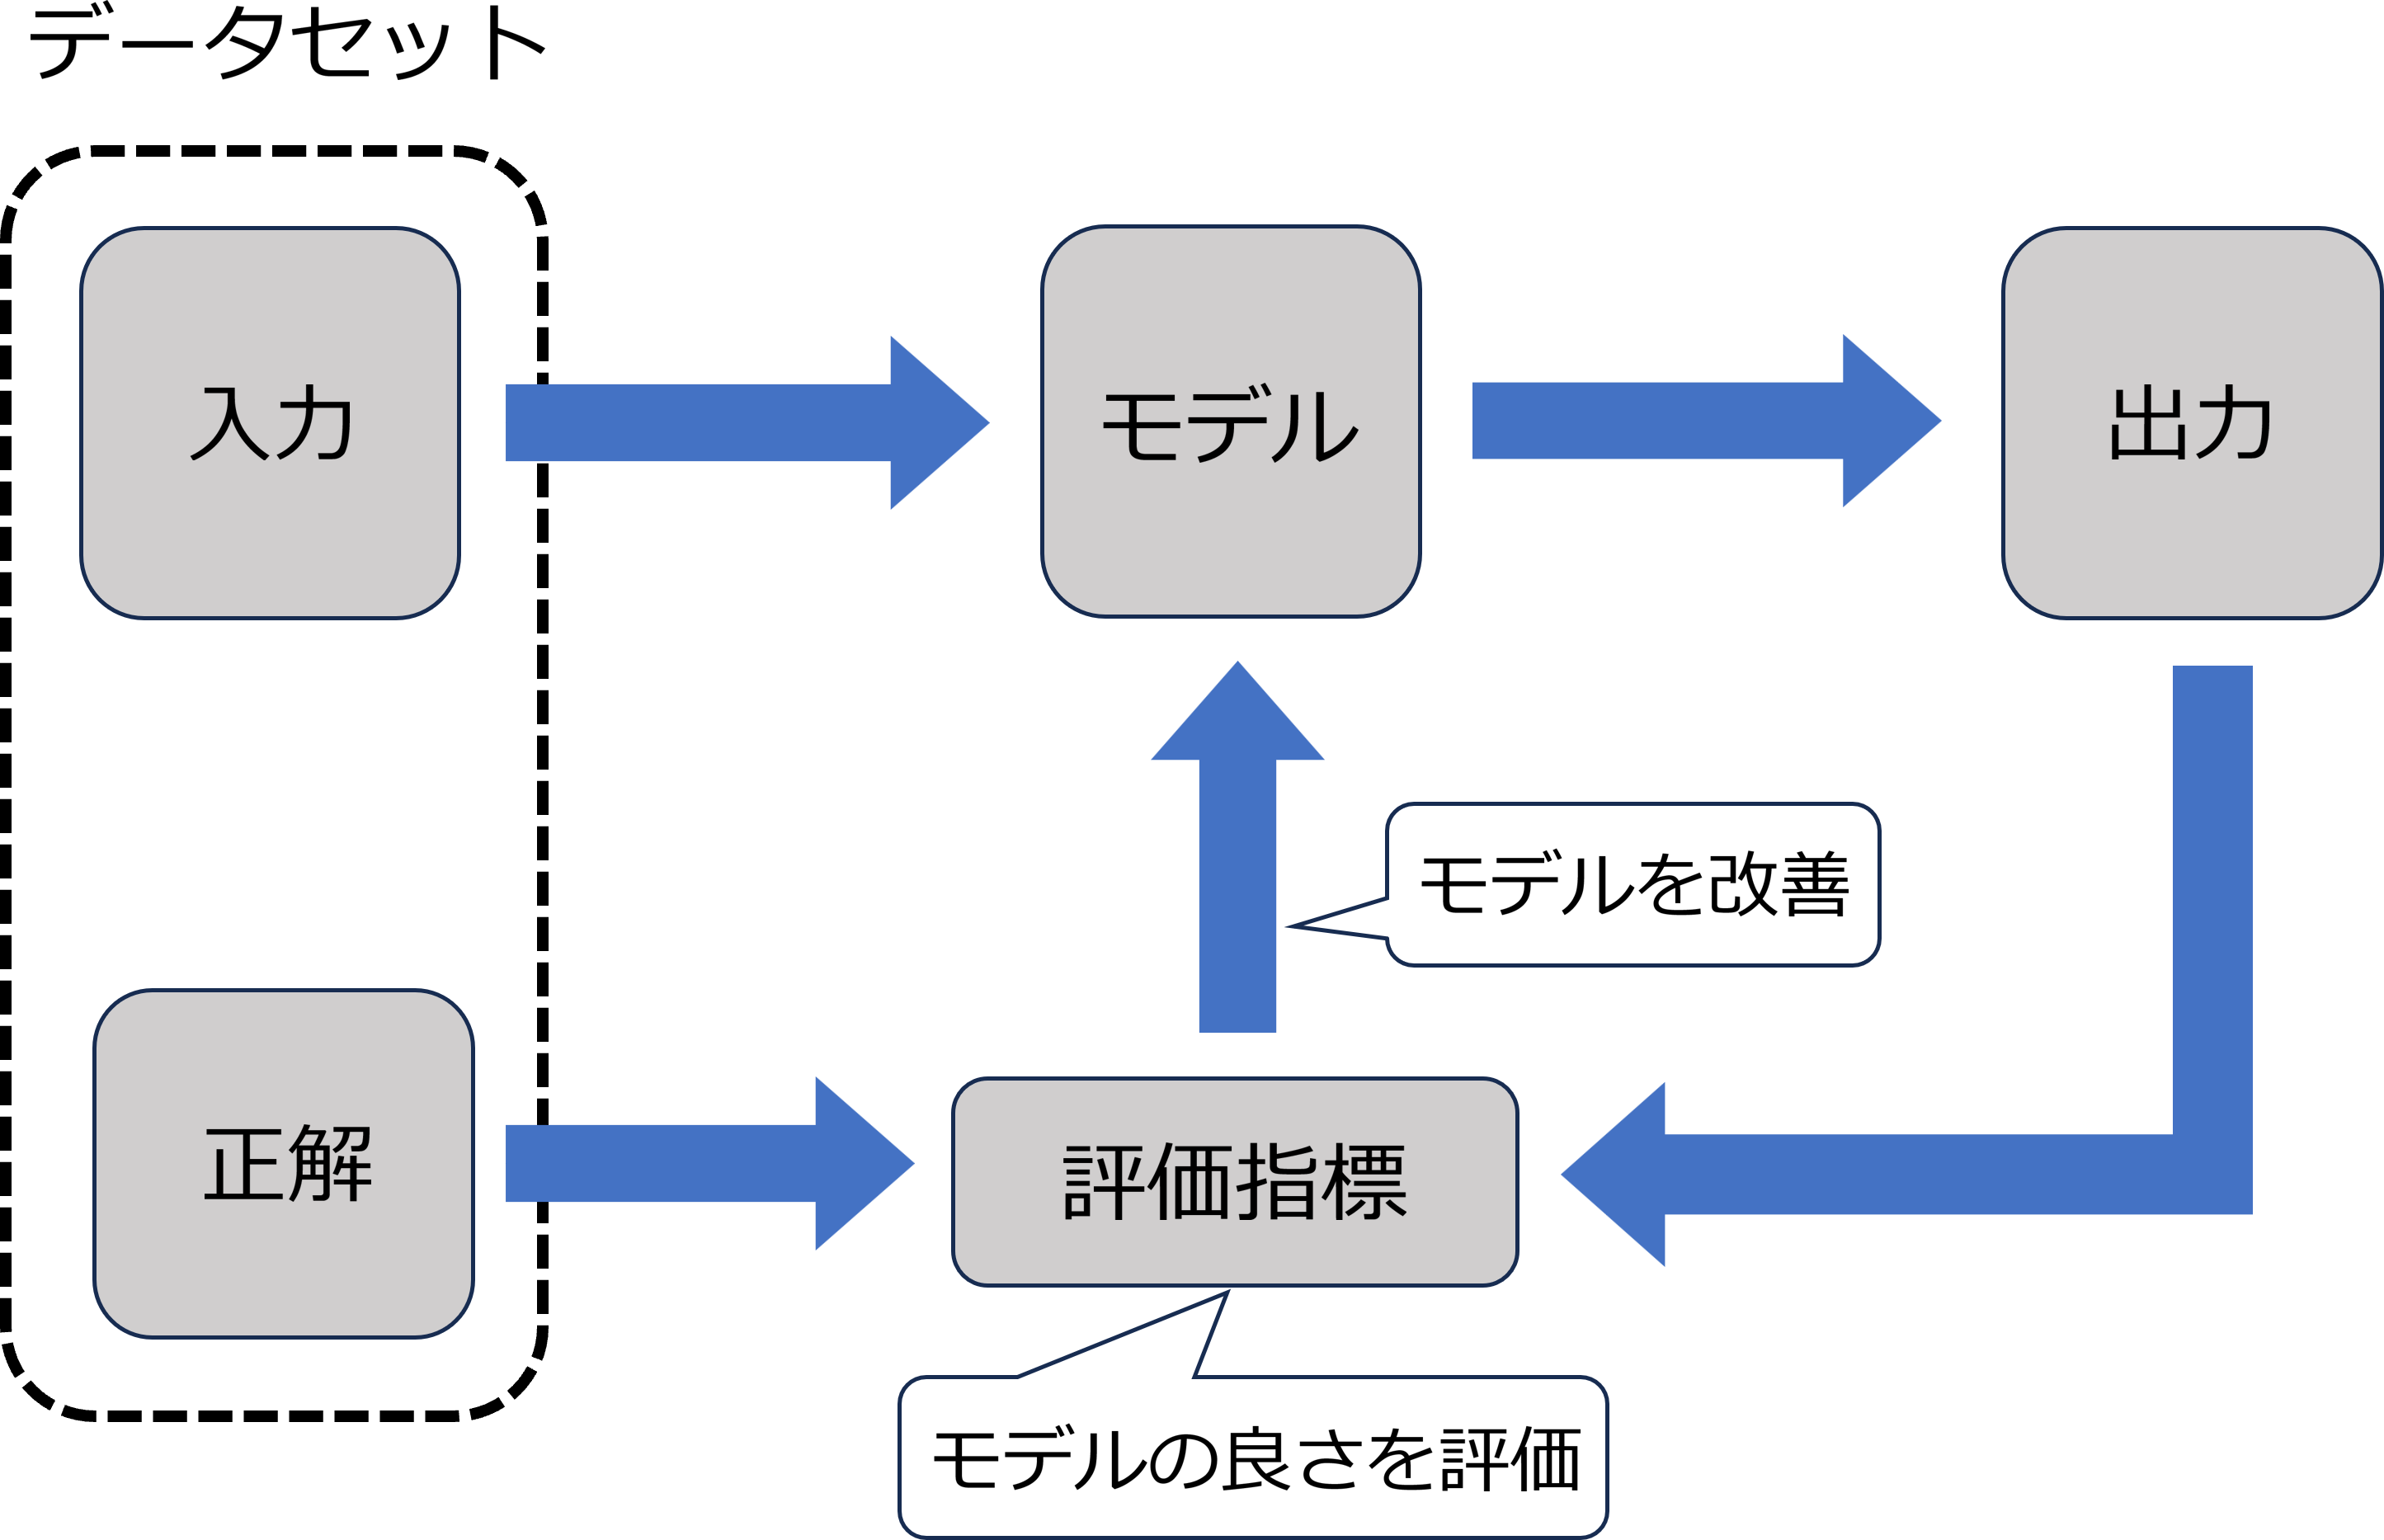
\includegraphics[height=6cm]{image/機械学習概要図.png}
    \caption{機械学習の大まかな流れ}
  \end{center}
\end{figure}
メトロポリス法とメトロポリス・ヘイスティング法は同じですか
\subsection{代表的なタスク}
ここでは,機械学習で解きたい問題であるタスクの代表的な例として「クラス分類」と「回帰」を紹介する.
\subsection*{クラス分類}
分類(classification)とは,データをいくつかのクラスに仕分ける作業のことである.例えば送られてきた電子メールをみて,それがスパムメールか通常メールを判別するような作業は,2クラス分類と呼べる.ここでのクラスというのは「スパムメールor通常メール」といった分類先のことを指す.ここで,スパムメールを$C_0$,通常メールを$C_1$とラベル付けしよう.また,入力データを$\bm{x}$とする.このとき,クラス分類というのは,与えられた$\bm{x}$が$C_0$と$C_1$のどちらに属するかを決定する作業である.数値的な変数$y = 0, 1$を導入すると,$\bm{x}$をクラス$C_{y}$へ分類するということは,$\bm{x}$の所属クラスを表す離散ベクトル$y(\bm{x})$の値を決めることであると言い換えられる.
\begin{equation}
  \bm{x} \longrightarrow y(\bm{x}) \in \{0, 1\}
\end{equation}
分類先のクラスが多数にわたる場合,多クラス分類とよび,分類先が$C_1,C_2,\dots,C_K$となり,ラベル$y(\bm{x})$も$1$から$K$の整数値をとる.これは先ほどの例でいえば,電子メールを「仕事」「家族」「友人」「スパム」と複数のファルダに分けることに対応する.
\subsection*{回帰}
データに対するクラス$y$は離散的とは限らない.例えば,過去数日の気象データ$\bm{x}$から明日の気温を予測したとき,$y$は温度の数値に相当し,連続的な実数値をもつ変数になる.このようにデータから,それに対応する実数値(を並べたベクトル)$\bm{y}$を予測作業のことを回帰(regression)という.つまり,回帰とは,与えられた$\bm{x}$を,対応する$\bm{y}$に変換するために関数$\bm{y}(\bm{x})$を決定する作業である.
\begin{equation}
  \bm{x} \longrightarrow \bm{y}(\bm{x}) \in \mathbb{R}
\end{equation}
\par
回帰による応用的なタスクとして,言語を翻訳する機械翻訳や音声を文字に起こす音声認識,状況が通常と異なることを自動的に検知させる異常検知,データのサイズを圧縮させるデータ次元削除などがあげられる.

\section{統計入門}
機械学習とは,データ(経験)をもとにしてプログラムがいろいろなタスクをこなせるようにさせることであった.ではどのようにしたらプログラムはデータからタスクをこなすための知識を学びとれるか?データを科学的に分析する数理的手法といえば,統計学である.機械学習の手法もまた統計を基礎として構築される.そのような視点から特に統計的機械学習と呼ばれている.ここではまず,統計の基礎を確認し,どのようにして学習アルゴリズムや評価指標を設計できるかについて説明する.
\subsection{標本と推定}
まず,データ(集合)(data(set))やサンプル,標本(sample)という用語についてきちんと定めておく.これらはデータ点(data point)の集まりからなる.手書き文字による画像認識の例でいえば,データは統計分析に用いるために用意した画像の集合のことで,1枚1枚の画像がそれぞれデータ点とよばれる.ただしデータ点も略してデータとよばれる.さらにはサンプルをサンプルの要素であるデータ点の意味でも用いられる.これらは用語の乱用であり,全く正しくない用法であるが,しばしば用いられているのが現状であるため,本論文でも文脈に応じてこの使い方に準じることにする.\par
このようなデータ点(サンプル)の集まりからなるデータを分析するのが統計である.ここでは推定について考える.まず統計解析に用いるデータは,母集団から抽出(sampling)されたものとみなす.データの要素を1つ取り出すことは,正確には抜き取り(draw)という.そしてデータの分析から,データ自身ではなくその背後にある母集団についての知識を獲得することを目標とする.これは例えば疫学者が飲酒量と健康の関係を調べたいときに,地球上のすべての(=母集団)を調査する必要はないということと同じである.その代わりにランダムに選び取った(抽出した)少人数に対する調査結果(データ)を分析することで,人類すべてに通用する飲酒量と健康の相関関係を読み取ろうとするということである.\par
母集団の性質はデータ生成分布(generative distribution)$P_{\text{data}}(\mathrm{x})$により特徴づけられているものとする.つまり,不確実性を伴う現象を確率的にモデル化するということである.

\subsection{教師あり学習と教師なし学習,強化学習}
機械学習には大きく3つに分類することができる.それは教師あり学習と教師なし学習,そして強化学習である.そのうち,ここでは本研究に関係する教師あり学習と教師なし学習について説明する.
\subsection*{教師あり学習}

\subsection*{教師なし学習}

\section{深層学習とは}
\subsection{ニューラルネットワーク}
\subsection{畳み込みニューラルネットワーク}
\section{ボルツマンマシンの基礎}

\chapter{イジング模型の相転移検出に関する研究}
\section{相の分類器による相転移検出}
\section{温度測定器による相転移検出}
\section{相転移検出がなせ可能なのか?}

\chapter{機械学習と繰り込み群}
\section{繰り込み群と特徴抽出}


\chapter{まとめ}
研究のまとめを書く.

%=====================================================================================
\chapter*{謝辞} %章を付けずにタイトル表示
\addcontentsline{toc}{chapter}{謝辞} %章立てせずに目次に追加するおまじない
謝辞を書く.

%=====================================================================================

% \addcontentsline{toc}{chapter}{参考文献} %章立てせずに目次に追加するおまじない
\renewcommand{\bibname}{参考文献} %これがないと,タイトルが「関連図書」になってしまう
\bibliography{reference} %bibtexファイルの読み込み
\bibliographystyle{junsrt} %本文に\cite{}を入れることで,参考文献表示

% 付録
\appendix
\renewcommand{\thechapter}{\Alph{chapter}}
\renewcommand{\thesection}{\Alph{chapter}.\arabic{section}}
\setcounter{section}{0}
\renewcommand{\theequation}{\Alph{chapter}.\arabic{equation}}
\setcounter{equation}{0}

\chapter{aaa}
aaa
\section{bbb}
bbb


\end{document}